%\documentclass[10pt,twocolumn, nofootinbib]{revtex4-2}
\documentclass[twocolumn,prl,floatfix,superscriptaddress]{revtex4-2}

\usepackage{amsthm, amsmath, amssymb, enumitem, graphicx, hyperref}
\usepackage{graphicx, subfigure}
\setlist{noitemsep}
\hypersetup{
	colorlinks=true,
	citecolor=blue,
	urlcolor=blue,
	linkcolor=blue
}
\urlstyle{same}

%\usepackage{graphicx, subfigure, amsfonts,amssymb,amsmath, array, gensymb,fontenc,color,lipsum}
%\documentclass[aps,twocolumn,showpacs,preprintnumbers]{revtex4}
%\usepackage{graphicx}  % Include figure files
%\usepackage{subfigure}
%\usepackage{multirow}
%\linespread{1.0}
%\usepackage{fancyhdr}
%\usepackage{longtable}
%\usepackage{parskip}
%\usepackage[T1]{fontenc}
%\usepackage{dcolumn}
%\usepackage{bm}        
%\usepackage{amsfonts}  
%\usepackage{amsmath}   
%\usepackage{amssymb}
%\usepackage{hyperref}
%\hypersetup{colorlinks= true, allcolors=blue}
%\setcitestyle{aysep={}}
%\setlength{\parindent}{11pt}
\frenchspacing


\begin{document}

\title{On the reality of the quantum state once again}
\author{Gabriele Carcass}
\affiliation{Physics Department, University of Michigan, Ann Arbor, MI 48109}
\author{Andrea Oldofredi}
\affiliation{Department of Philosophy, University of Lisbon, Portugal}
\author{Christine Aidala}
\affiliation{Physics Department, University of Michigan, Ann Arbor, MI 48109}
\vspace{2mm}

\date{\today}


\begin{abstract}
The ontological model framework introduced by Harrigan and Spekkens has been widely used to categorize quantum interpretations and as a basis for influential results such as the PBR theorem. In this paper we show that the model has a fundamental flaw: the epistemic structure it implicitly assumes does not follow the one dictated by quantum mechanics. Namely, the map between the epistemic states of the model and quantum density matrices is not even an order homomorphism in terms of the information entropy, consequently the epistemic content of mixed states is not mapped in a meaningful way. Moreover, by recasting the definitions of the model in terms of density matrices, we find that only $\psi$-epistemic interpretations are allowed by quantum mechanics, a result that is the opposite of the PBR theorem. We show that the cause of this mismatch is the effect of non-contextuality over mixed preparations that does not allow for a single decomposition of mixed states over pure states.
\end{abstract}

\maketitle

\section{Introduction}

%- Status of field and impact of HS
%- Mention the PBR Theorem explicitly
%- Claim that HS does not work for quantum epistemic cases, therefore invalidating all results


\section{Summary of the Harrigan \& Spekkens Model}

\subsection{Ontological Models}

Harrigan and Spekkens (HS) provide a classification of ontological quantum models that essentially depends on the nature of the quantum state \cite{Harrigan:2010}. Such ontological models are defined by employing an operational setting where the primitive of descriptions consist in preparation protocols and measurements performed on quantum systems. More precisely, HS claim that preparations procedures are ``assumed to prepare a system with certain properties and a measurement procedure is assumed to reveal something about those properties'' (\cite{Harrigan:2010}, p.\ 128). In their approach the complete specification of the attributes of a given physical object is provided by $\lambda$, the ontic state of the system under scrutiny. Such operational models provide the probabilities $p(k|M, P)$ to obtain outcomes $k$ for some measurement $M$ performed on the prepared systems, given the set of preparation instructions $P$. Indeed, from a formal perspective every protocol $P$ is associated with a density operator $\rho$ on the relevant Hilbert space, and every measurement $M$ is associated with a POVM $\{ E_k\}$. As usual, each measurement result $k$ can be obtained with probability $p(k|M, P)=\textrm{Tr}(\rho E_k)$, the generalized Born rule. To this regard, HS underline that although an agent perfectly knows the preparation procedures prior the performance of a certain measurement, they may have incomplete knowledge of $\lambda$. This is means that an observer which has incomplete information about $\lambda$ assigns ``non-sharp'', i.e.\ overlapping probability distributions $p(\lambda| P)$ over $\Lambda$, the space of ontic states. 

We can eventually provide the formal definition of ontological models as follows (\cite{Harrigan:2010}, p.\ 128): ``An ontological model of operational quantum theory posits an ontic state space $\Lambda$ and prescribes a probability distribution over $\Lambda$ for every preparation procedure $P$, denoted $p(\lambda| P)$, and a probability distribution over the different outcomes $k$ of a measurement $M$ for every ontic state $\lambda \in \Lambda$, denoted $p(k|\lambda, M)$. Finally, for all $P$ and $M$, it must satisfy
\begin{align*}
\int d\lambda p(k|\lambda, M) p(\lambda| P)= \textrm{tr}(\rho E_k),
\end{align*}
\noindent where $rho$ is the the density operator associated with $P$ and $E_k$ is the POVM element associated with outcome $k$ of $M$''.

\subsection{$\psi-$ontic and $\psi-$epistemic models}

Let us now introduce the first categorization of ontological models. HS divide them in $\psi-$\emph{complete} and $\psi-$\emph{incomplete}: in the former case, the quantum state encodes every information about the physical system at hand, as in the case of standard Quantum Mechanics (QM). Alternatively stated, in $\psi$-complete models there is a one-to-one relation between pure quantum states and the ontic state of physical items they represent. Formally, this is translated into the following definition (\cite{Harrigan:2010}, p.\ 131): ``An ontological model is $\psi-$complete if the ontic state space $\Lambda$ is isomorphic to the projective Hilbert space $\mathcal{PH}$ (the space of rays of Hilbert space) and if every preparation procedure $P_{\psi}$ associated in quantum theory with a given ray $\psi$ is associated in the ontological model with a Dirac delta function centered at the ontic
state $\lambda_{\psi}$ that is isomorphic to $\psi$, $p(\lambda|P)=\delta(\lambda-\lambda_{\psi})$''.
In the latter case, $\psi$ alone is not sufficient to provide a complete description of reality. Models in which $\psi$ is supplemented with additional/hidden variables are defined by HS as $\psi-$supplemented (well-known examples are Bohm pilot-wave theory \cite{Bohm:1952aa} and Nelson mechanics \cite{Nelson:1966aa}). 

In the second place, the authors propose another distinction concerning the nature of quantum states, classifying $\psi$ either as \emph{ontic} or \emph{epistemic}. In a nutshell, a model is said to be $\psi-$ontic if ``for any pair of preparation procedures, $P_{\psi}$ and $P_{\phi}$, associated with distinct quantum states $\psi$ and $\phi$, we have $p(\lambda | P_{\psi})p(\lambda|P_{\phi})=0$ for all $\lambda$'' (\cite{Harrigan:2010}, pp.\ 131-132). Consequently, (i) in $\psi-$ontic models the ontic state $\lambda$ can be consistently described only by a unique pure quantum state $\psi$, and (ii) observers' epistemic states associated with different quantum states are non-overlapping in $\Lambda$, i.e.\ they correspond to disjoint regions of the space of ontic states. Alternatively, in $\psi-$ontic models different pure quantum states correspond to disjoint probability distributions $\mu$ over $\Lambda$ (cf.\ Figure 1a). 

If a model in not $\psi-$ontic, then it is $\psi-$epistemic. A model is defined $\psi-$epistemic if $\lambda$ can be described by more than one quantum state. Therefore, in such epistemic models there are quantum states that correspond to overlapping probability distributions over $\Lambda$ (cf.\ Figure 1b).
This fact implies that agents' epistemic states overlap, i.e.\ there exist preparation procedures $P_{\psi}, P_{\phi}$ and a $\lambda\in\Lambda$ such that $p(\lambda | P_{\psi})p(\lambda|P_{\phi})\neq0$. In turn, this entails that the ontic state $\lambda$ can be consistently represented by both quantum states $\psi$ and $\phi$: ``[i]n a $\psi-$epistemic model, multiple distinct quantum states are consistent with the same state of reality---the ontic state $\lambda$ does not encode $\psi$'' (\emph{ibid.}, p.\ 132). This explains why the authors claim that in $\psi-$epistemic models quantum states refer to observers' incomplete knowledge of reality, and not to reality itself.

\begin{figure}
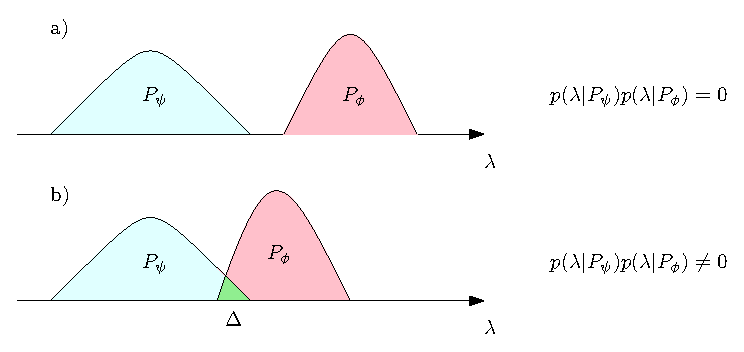
\includegraphics[scale=.7]{ontic}
\caption{\footnotesize{Harrigan and Spekkens distinction between $\psi-$ontic (a) and $\psi-$epistemic (b) ontological models.}}
\end{figure}

Now we can combine both distinctions in order to classify different ontological models. As we have seen, in $\psi-$complete models there is a one-to-one relation between $\lambda$ and its description provided by $\psi$. Consequently, if one knows the quantum state $\psi$ then one has a complete knowledge of the ontic state $\lambda$ of the system under consideration. In this models a variation of $\psi$ implies a variation of the ontic state, therefore $\psi-$complete models are $\psi-$ontic. If ontological models are $\psi-$incomplete, then they may be either $\psi-$supplemented or $\psi-$epistemic. In the former case the description of a physical system provided by $\psi$ is incomplete and is supplemented with additional (or hidden) variables whose value is generally unknown. Notably, also the class of $\psi-$supplemented models is $\psi-$ontic. Finally, in $\psi-$epistemic models $\psi$ represents an agent's incomplete knowledge of reality (of $\lambda$), and not reality itself; in this case a variation of $\psi$ does not necessarily entail a variation of $\lambda$.

From these distinctions some conclusions can be inferred. In the first place, models which are simultaneously $\psi-$complete \emph{and} $\psi-$epistemic cannot exist. Therefore, if a model is $\psi-$complete, it must be $\psi-$ontic (cf.\ Lemma 6, \cite{Harrigan:2010}, p.\ 133). Alternatively, if a model is $\psi-$incomplete, then it can either be $\psi-$ontic, as in the case of $\psi-$supplemented models, or $\psi-$epistemic. If a model is $\psi-$epistemic, then it cannot be $\psi-$ontic, since it does not describe any underlying physical reality, but only the agents' knowledge of it. 


\section{Quantum epistemic states}
Now that we have presented the model, we want to study the space of epistemic states. To make the discussion more concrete, we will assume we have a $\psi$-complete ontological model of a single qubit representing the direction of spin.

Suppose we have two preparation devices, one that prepares z+ and another that prepares z-, and we toss a fair coin to choose which one to use. This results into an epistemic state with equal distribution on z+ and z-. Now suppose we have two additional preparation devices, this time for x+ and x-, and we again toss a fair coin. This time we have an epistemic state with equal distribution on x+ and x-. Note that the epistemic distributions do not overlap. Therefore, according to the HS categorization, these correspond to two ontologically distinct states, making the preparation axis an ontological property of the system, regardless of the orientation. However, in terms of density matrixes both these situations would not just overlap: they would be represented by the same maximally mixed state. Hence there seems to be a mismatch between the type of epistemic knowledge one can express in quantum mechanics through mixed states and the type of epistemic knowledge described in the HS model. This needs to be investigated further.

Let us first characterize the extent of the discrepancy. In HS, the space of epistemic states $E_{HS}$ is the set of probability distributions over pure states, which is an infinite dimensional space. This is a direct consequence of defining the epistemic states as a distribution $P(\lambda|P)$ that, for each preparation $P$, assigns a well defined probability to each ontological state $\lambda$.\footnote{TODO: HS seems to be very vague about probability and probability density.} In QM, mixed states $E_{Q}$ are in one-to-one correspondence with the interior of the Bloch sphere, a three dimensional manifold. Looking at the difference in dimension, the discrepancy is not minor.

Note that the space of pure states $\Lambda$ is the same in both cases, one state for each direction of spin. Also note that all epistemic states in both spaces can be reached by mixture of pure states. The difference is that, in the quantum case, we have an ``aliasing'': different mixtures will give the same mixed states. Since each classical probability distribution corresponds to a unique mixing of pure states, we have a map $\iota : E_{HS} \mapsto E_{Q}$ that allows us to go from HS epistemic states to density matrixes. This map is surjective but not injective. Therefore $E_{Q}$ can be seen as a set of equivalence classes of $E_{HS}$. The key question, then, is the following: is the map $\iota$ sufficiently well behaved that we can understand the epistemic content of $E_{Q}$ based on the epistemic content of $E_{HS}$? Or is it so hopelessly broken that there is no connection between the two?

Ideally, one would like to say is that $E_{HS}$ represents all possible epistemic states that include the knowledge about preparation, while $E_{Q}$ represents only those distinguishable through measurement. For example, one may want to say that the axis of preparation is, in principle, an ontologically distinct property, but this is not experimentally distinguishable. Therefore distinct epistemic states for each direction are projected by $\iota$ onto the same epistemic state of maximum uncertainty. This sounds very plausible and appealing, but it turns out this is not at all the case. To show this we will concentrate on a single aspect about the map: how information entropy transforms under the map. While there are other problems, we do not need to explore them: given the crucial role of entropy in information theory, its breakdown is sufficient to claim that the epistemic structures of $E_{HS}$ and $E_{Q}$ are different.

Since every pure state in quantum mechanics has zero entropy, we will assume that this is the case for all pure states in $E_{HS}$. Let us consider three uniform distributions over a sphere with support given by:
\begin{description}
	\item[A] the poles, z+ and z-
	\item[B] the equator, all states on the x/y planes
	\item[C] the whole sphere, all points
\end{description}
Since we want the entropy for a single microstate to be zero, the entropy for A will be 1 (uniform distribution between two discrete cases). Since $\iota(A)$ will be the maximally mixed state, which also corresponds to entropy 1. So far so good: $\iota$ maps entropy 1 to entropy 1! However, note that A is a measure zero set of B, which is a measure zero set of C. The entropy of C is therefore infinite with respect to B which is infinite with respect to A. On the other hand, A, B and C will all correspond to the same maximally mixed state, therefore $\iota$ collapses together epistemic states at different level of infinity. Note that, in this case, $\iota$ picks the minimum entropy between the equivalent epistemic states. This is inconsistent with the idea that $E_{Q}$ represents states where knowledge is lost: that would pick the maximum possible entropy.

\begin{figure}
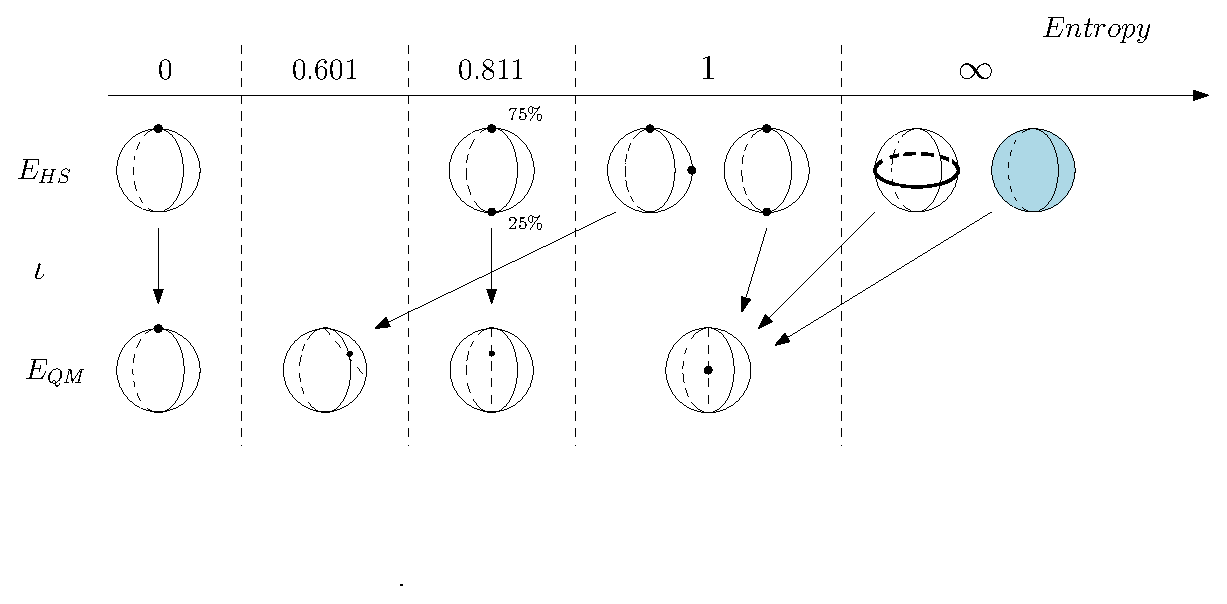
\includegraphics[scale=.4]{fig2}
\caption{\footnotesize{}}
\end{figure}

Now consider another uniform distribution over the support:
\begin{description}
	\item[D] the north pole and a point on the equator, z+ and x+.
\end{description}
This is yet another uniform distribution between two discrete cases, therefore in $E_{HS}$ the entropy is 1. However, $\iota(D)$ is not the maximally mixed state and therefore the entropy is less than 1. This means that epistemic states that are isoentropic in $E_{HS}$ are not isoentropic $E_{Q}$. If we think as $E_{HS}$ and $E_{Q}$ as partially ordered by information entropy, then $\iota$ is not an order preserving map. Therefore the epistemic structures represented by $E_{HS}$ and $E_{Q}$ are not isomorphic.

The seemingly innocuous assumption that $P(\lambda|P)$ is well defined for all preparations $P$ and for all states $\lambda$ imposes a classical probability space which follows the rules of classical information theory, and prevents the state space $\Lambda$ to support an epistemic structure compatible with quantum theory. This suggests an obvious follow up: what if we start by assuming that the set of pure states $\Lambda$ supports the correct epistemic structure, the one associated with density matrices, and use the same definitions of $\psi$-ontic and $\psi$-epistemic?

The difficulty here is that support and overlaps are not a well defined concept for density matrices. Yet, there are two different properties that non-overlapping functions have in classical probability theory. Two distribution $\rho_1$ and $\rho_2$ are non-overlapping if and only if:
\begin{enumerate}
	\item their product $\rho_1 \rho_2 = 0$ is zero
	\item the probability of being in the support of the second given the first is zero.
\end{enumerate}
In quantum mechanics, if we consider two pure states $\psi_1$ and $\psi_2$, they lead to the following conditions:
\begin{enumerate}
	\item $|\psi_1><\psi_1|\psi_2><\psi_2| = 0$
	\item $<\psi_2|\psi_1><\psi_1|\psi_2> = 0$.
\end{enumerate}
Both of these are satisfied if and only if $<\psi_1|\psi_2>=0$: the states are non-overlapping if and only if they are orthogonal. This is, not suprisingly, exactly what happens in classical probability: two distributions are non-overlapping if and only if they are orthogonal with respect to the inner product $\int \rho_1 \rho_2 d\lambda$.\footnote{We could also define the overlap in terms of the entropy of the mixture and we would find the same result.}

Therefore we have the following result: if we want a set of pure states that are able to support the epistemic structure of quantum mechanics, they must be ``overlapping'' and therefore they cannot be take to be ontic. The reader is no less entitled to conclude that quantum mechanics does not allow $\psi$-ontic interpretations from this result than he would be entitled to conclude that quantum mechanics does not allow $\psi$-epistemic interpretations from PBR. He would also be entitled to conclude that the categorization is flawed.


%- Try to apply their model to a purely mixed state of spin 1/2
%- Show that you can't have a single epistemic distribution
%-> Failure of model

\section{Discussion}

Let us now step back a moment. Why does assuming $p(\lambda|P)$ lead to an epistemic structure incompatible with the quantum one?

It is widely understood that one feature of quantum mechanics is non-contextuality: a measurement cannot be understood as revealing pre-existing values. We may be tempted to think that we have one context before and one after the measurement. What we are seeing that this does not work because we a dual effect on preparations. As we cannot understand quantum measurements as selecting from a single joint probability distribution, we cannot understand quantum preparations as constructing a single joint probability distribution. To fully understand how this works, let us review how how probability spaces work in both classical and quantum mechanics.

A ``classical'' probability space is made of three objects: a sample space $\Omega$ which represents all possible cases (e.g. all points in phase-space for a classical system); a $\sigma$-algebra $\Sigma_\Omega$ over $\Omega$ which represents all statements of interest (e.g. ``the position is between 2 and 3 meters''); a measure $\mu : \Sigma_\Omega \to \mathbb{R}$ that associates each statement with a probability. Note how we have a single probability distribution over the whole space.

In quantum mechanics we start with a similar structure: a set of states $\mathcal{H}$ which represents all possible cases (i.e. the Hilbert space) and a $\sigma$-algebra $\Sigma_{\mathcal{H}}$ that represents all statements of interests. This is where the similarity ends. To specify a mixed state, a ``quantum distribution'', we use a density matrix $\rho : \mathcal{H} \to \mathcal{H}$. To get a probability distribution, we need to specify an observable $O$. The observable $O$ identifies an orthogonal basis and we take the sub-algebra $\Sigma_O \subset \Sigma_{\mathcal{H}}$ defined on those states. We can then associate $\Sigma_O$ with a measure $\mu_O : \Sigma_O \to \mathbb{R}$, which is therefore not on the whole space $\Sigma_{\mathcal{H}}$.

Mathematically, what we call context is a $\sigma$-algebra: a set of propositions upon which we assign probabilities. This tells us why we cannot simply use classical rules in quantum mechanics. Classical mechanics has only one context, so we can always mix and match statements however we please. In quantum mechanics, propositions about different observables live in different $\sigma$-algebras, in different probability spaces, and therefore cannot be combined.

One may think that we can get away by assuming that, at each time, there is a ``true'' context. And this seems to work in some cases. Given any density matrix $\rho$, there exist a (non-unique) privileged context: this is the one in which we can express $\rho = \sum p_i |\psi_i > < \psi_i|$ as the mix of orthogonal pure states. If $\rho$ is itself a pure state, any basis that includes it will be a privileged context. This privileged context provides us the probability distribution over which the information entropy is calculated. After a measurement, the privileged context changes to one that includes the eigenstates of the chosen observable. However, this does not work in general.

Suppose we start with two density matrixes $\rho_1$ and $\rho_2$ with different eigenstates. We then create the mixture $\rho = p_1 \rho_1 + p_2 \rho_2$. The contexts of the mixture will not be the same as the original contexts. It will, in fact, even depend on $p_1$, $p_2$. That is, when mixing preparations we are not simply combining two probability distribution over the same context, like in classical mechanics, but we are combining the contexts themselves. Non-contextuality does not affect only measurement, but, dually, preparations as well. And this affect how information entropy is calculated and the overall epistemic structure.

% TODO: mention tomography?

To sum up, assuming $p(\lambda|P)$ exists means assuming there is a single probability space, a single $\sigma$-algebra, a single set of propositions, to which all probabilities are assigned. This is exactly assuming non-contextuality. While this can be made to work for pure state to pure state transitions during measurement, mixing preparations leads to an epistemic structure that is fundamentally non-contextual, leading to inconsistencies with quantum mechanics. To allow for contextuality we should assume that for each observable $O$ we have a probability $p_O(\lambda_O|P)$ of having prepared one of the eigenstates, such that $\sum_{\lambda_O} p_O(\lambda_O|P) = 1$. The entropy of the preparation would be the lowest entropy across all contexts.


% (mezza pagina)
%- Non-contestuality of HS
%- PBR and other results

\section{Conclusion}

%\section*{Supplementary material}
%
%TODO: do we need to bump anything here?


\bibliographystyle{apalike}
\bibliography{PhDthesis}


\end{document}